
\documentclass[12pt]{article}
\usepackage{geometry} % see geometry.pdf on how to lay out the page. There's lots.
\geometry{a4paper} % or letter or a5paper or ... etc
% \geometry{landscape} % rotated page geometry
\usepackage{graphicx}
% See the $$Article customise'' template for come common customisations

\title{Scaling Erasure codes with integrity audits}
\author{Viktor Trón}
\date{PhD thesis. draft of \today} % delete this line to display the current date
\pagestyle{plain}
\pagenumbering{arabic}
% \usepackage{color}\
\usepackage{amsmath}
\bibliographystyle{apalike}
%%% BEGIN DOCUMENT
\begin{document}

\maketitle
\tableofcontents

\begin{abstract}
This paper brings together two problem areas of computer infrastructure, coding theory and proof of custody to tackle the scaling of erasure codes in the context of a distributed storage system. We offer a double divide and conquer approach: we encode the data in a (merkle) tree and apply erasure code to each set of children, this spacial division trades off reliability for linear coding performance. On the other hand we refine the underlying loss model by arbitrary temporal resolution and conquer by showing repeated recursive audits when done frequently can counterbalance for the degree of reliability lost on the way. This technique shifts the quadratic complexity of the erasure codes to a background process and thereby significantly improving on the practical data size limitations inherent in erasure codes.
\end{abstract}

\section{Introduction}

Erasure codes and proofs of custody, though somewhat related, are not commonly mentioned in one sentence given they are typically used at very different application areas. Coding theory offers a solution to problems of data loss, improving data availability and reliability of data storage systems; while proof of custody is concerned with offering cryptographic contructs that allow custodians of data to prove to third parties that they have the data available.
Both constructions proved to be useful (and indeed complementary) in the process of designing and implementing swarm, a decentralised serverless hosting platform, a distributed storage network and content delivery service infrastructure \cite{ethersphere2016sw3}.

Swarm uses a content addressed storage over a network of nodes. Content addressed storage is crucial in organising retrieval and distribution of data chunks and solves the problem of eliminating unneccesary replication since data is stored at the address that is deterministically derived from the data itself. By choosing the address function to be irreversible and pseudorandom the system is capable of integrity protection and allows for efficient key-based routing protocols \cite{maymounkov2002kademlia}.

While eliminating unessessary replication is a desireable feature in a storage network, in order for such networks to be used in the real word, they must still be able to offer resilience in the face of various infrastructual failings. Most notably, some level of redundancy of data storage is essential to a zero-downtime, low-latency, fault-tolerant network. Erasure coding is a well known technique to implement redundant storage and therefore was a natural choice.

\section{Erasure codes}

Erasure codes are commonly used to ensure that data is available even if parts of the storage system are faulty. In particular they allow us to constuct storage schemes (data encoding and distribution) that solves this problem more efficiently than simple replication.  The problem is framed in the context of guaranteeing some probability that the data is retrievable given some model expressing the expected fault conditions in the storage subsystems.
Coding theory in practice is often concerned with RAID-s and computer hardware architecture synchronising disks for resilient datacentre storage.
Erasure codes in particular see the problem as how to encode data into shards distributed across $n$ disks so that the data is fully retrievable in the face of a particular probability that one disk is faulty.
Similarly in the context of a distributed chunkstore, the problem can be recouched as the question how to encode the data into chunks distributed across the nodes in the network so that the entire data is retrievable in the face of a particular probability that one chunk is missing\footnote{The distributed chunkstore model uses fixed-sized chunks which are either completely lost or completely undamaged. Since the swarm content storage uses the hashes of chunks as their addresses, and since the chunks are stored by custodian nodes that are randomly distributed in the same address space, we are safe to assume that the storage allocation is independent of all the other nodes and data. This assures that recovering a chunk at any point can practically be thought of as failing with equal and independent probability.}


The Cauchy-Reed-Solomon erasure code (henceforth CRS, \cite{lubyetal1995CRS}, \cite{plank2006optimizing}) is a \emph{systemic erasure code} which applied to a data blob of $m$ fixed-size pieces, produces $k$ extra pieces (so called \emph{parity pieces}) of the same size in such a way that any $m$ out of $n=m+k$ fix-sized pieces are to enough to reconstruct the original blob. The storage overhead is therefore given by $\frac{k}{m}$.%
%
\footnote{%
There are open source libraries that implement Reed Solomon or Cauchy-Reed-Solomon coding. See \cite{plank2009performance} for a thorough comparison.}

%
% formula for probability of loss.
%

Both the encoding and the decoding of CRS codes takes $O(mk)$ time, where $n$ is the number of data chunks, $k$ is the number of additional chunks as well as the maximum number of chunks that can be lost without losing decodeability. If $k$ is defined as a given fraction of $m$, which is necessary for guaranteeing a certain probability of retrievability under the condition of a fixed probability $p$ of losing a single chunk, the time complexity of CRS codes becomes $O(n^2)$, which is utterly unacceptable for large files. %large files = large n only when chunk size is fixed.

\section{The swarm chunk tree}

Swarm uses hierarchical merkle tree \cite{merkle1980protocols} to reorganise data into fixed sized chunks which are then sent off to the swarm nodes to store (by a node close to their address which makes it retrievable by the hash (content address).
Assuming $h$ the size of the hash output of the hash function used in bytes, $b$ is the branching factor. Each node represents the root hash of a subtree or, at the last level, the hash of a $b\cdot h$ long span (one chunk) of the file. Generically we may think of each chunk as consisting of $b$ hashes:


\begin{figure}[htbp]
   \centering
   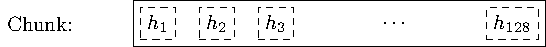
\includegraphics{fig/chunk.pdf} % requires the graphicx package
   \caption{A swarm chunk consists of 4096 bytes of the file or a sequence of 128 subtree hashes.}
   \label{fig:chunk}
\end{figure}

while in the tree structure, the 32 bytes stored at the node represent the hash of the 128 children.

\begin{figure}[htbp]
   \centering
   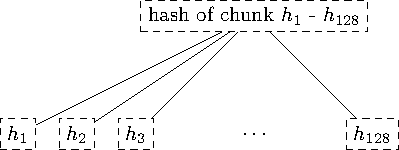
\includegraphics{fig/treebasic.pdf} % requires the graphicx package
   \caption{ A generic node in the tree has 128 children.}
   \label{fig:treebasic}
\end{figure}

During normal swarm lookups, a swarm client performs a lookup for a hash value and receives a chunk in return. This chunk in turn constitutes another $b$ hashes to be looked up in return for another $b$ hashes and so on until the chunks received belong to the actual document. Here is a schematic: (See Figure \ref{fig:tree2}).


\begin{figure}[htbp]
   \centering
   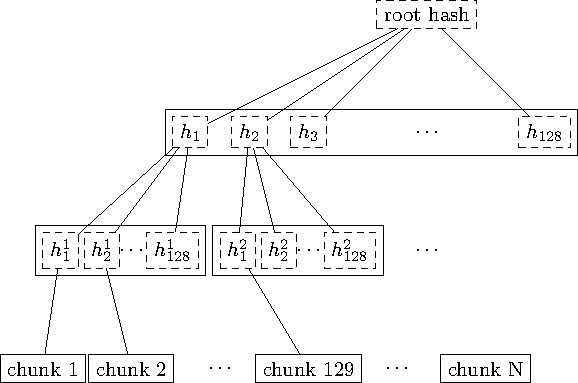
\includegraphics{fig/tree2.pdf} % requires the graphicx package
   \caption{ The swarm tree is the data structure encoding how a document is split into chunks.}
   \label{fig:treebasic}
\end{figure}

\section{Erasure codes and the swarm chunk tree}

While off-the-shelf erasure coding could be used on documents uploaded in swarm, this solution has immediate problems. Apart from the quadratic complexity of encoding, chunking the CRS endoded datablob with the chunker would result in certain chunks to be more vulnarable, since their retrieval is dependent on the retrieval of the chunks that encode all their ancestor nodes in the chunktree.

This prompted us to try and align the notion of swarm chunk with the chunk used in the CRS scheme. This led us to encode redundancy directly into the swarm tree by applying the \emph{CRS scheme}  to each set of chunks that are children to a node in the chunkree.

The \emph{chunker} algorithm using CRS coding work the following way when splitting the document:

 1. Set input to the data blob.
 2. Read the input one chunk (say fixed 4096 bytes) at a time. Count the chunks by incrementing $i$. The last chunk read may be shorter.
 3. Repeat 2 until there's no more data or $i \equiv 0$ mod $m$
 4. use the CRS scheme on the last $i \mod\ m$ chunks to produce $k$ parity chunks resulting in a total of $n \leq m+k$ chunks.
 . Calculate the hashes of all the these chunks and concatenate then to result in the next chunk (of size $i\mod m$ of the next level. Record this chunk as the next
 6. If there is more data repeat 2. otherwise
 7. If the next level data blob has more than one chunk, set the input to this and  repeat from 2.
 8. Otherwise remember the blob as the root chunk.

Assume we fix the branching factor of the swarm hash (chunker) as $n=128$ and $h=32$ as the size of the \emph{SHA3 Keccak hash}. This gives us a chunk size of $4096$ bytes.

Let us now suppose that we start splitting out input document data into chunks, and after each $m$ chunks then add $k=n-m$ parity check pieces using a Reed-Solomon code so that now any $m\text{-out-of-}n$ chunks are
sufficient to reconstruct the document. On the next level up the chunks are composed of the hashes of the $m$  data chunks and the $k$ hashes of the parity chunks. Let's take the first $m$
of these and add an additional $k$ parity chunks to those such that any $m$ of the resulting $n$
chunks are sufficient to reconstruct the origial $m$ chunks. And so on and on every level. In terms of
availability, every subtree is equally important to every other subtree at this level. The resulting
data structure is not a balanced tree since on every level $i$ the last $k$ chunks are parity leaf
chunks while the first $m$ are branching nodes encoding a subtree of depth $i-1$ redundantly.
A typical piece of our tree would look like this (see Figure \ref{fig:tree-with-erasure}).


\begin{figure}[htbp]
   \centering
   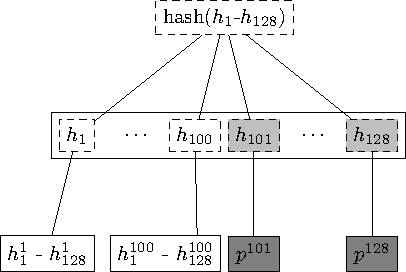
\includegraphics{fig/tree-with-erasure.pdf} % requires the graphicx package
   \caption{The swarm tree with extra parity chunks using $m$ out of 128 CRS code. Chunks $p^{m+1}$ through $p^{128}$ are parity data for chunks $h^1_1 - h^1_{128}$ through $h^{m}_1  - h^{m}_{128}$.}
   \label{fig:tree-with-erasure}
\end{figure}


This pattern repeats itself all the way down the tree. Thus hashes $h^1_{m+1}$ through $h^1_{128}$ point to parity data for chunks pointed to by $h^1_1$ through $h^1_{m}$.Parity chunks $p^i$ do not have children and so the tree structure does not have uniform depth.

If the number of file chunks is not divisible by $m$, then we cannot proceed with the last batch in the same way as the others. We propose that we encode the remaining chunks with an erasure code that guarantees at least the same level of security as the others. Note that it is not as simple as choosing the same redundancy. For example a 50-of-100 encoding is much more secure against file loss than a 1-of-2 encoding even though the redundancy is 100\% in both cases. Overcompensating, we could say that there should always be the same number of parity chunks even when there are fewer than $m$ data chunks so that we always end up with $m\text{-out-of-}n$. We repeat this procedure in every row in the tree.

This leaves us with only one corner case: it is not possible to use our $m\text{-out-of-}n$ scheme on a single chunk ($m=1$) because it would amount to $k+1$ copies of the same chunk. The problem of course is that any number of copies of the same chunk all have the same hash and are therefore indistinguishable in the swarm. Thus when there is only a single chunk left over at some level of the tree, we'd have to apply some transformation to it to obtain a second (but different) copy before we could generate more parity chunks.

In particular this is always the case for the root chunk. To illustrate why this is critically important, consider the following. The root hash points to the root chunk. If this root chunk is lost, then the file is not retrievable from the swarm even if all other data is present. Thus we must find an additional method of securing and accessing the information stored in the root chunk.

Whenever a single chunk is left over ($m=1$) we propose to append an extra padding byte to the chunk not counting towards its size. In swarm, each 4096 byte chunk is actually stored together with 8 bytes of meta information - currently only storing the size of the subtree encoded by the chunk. Since the subtree size determines exactly what span of the chunk is substantive data, the padding differential byte is easily ignored when the document is assembled.%
%
\footnote{%
Note that the typical values for $k$ will be in the single digits so a single byte will allways suffice. Note that in the special cornercase when the singleton leftover chunk is a full chunk, we end up having an oversized chunk.
}

\section{Scalability issues}

This per-level $m\text{-out-of-}n$ Cauchy-Reed-Solomon erasure code once introduced into the swarm chunk tree does not only ensure file availability, but also offers further benefits of increased resilience and ways to speed up retrieval \cite{ethersphere2016sw3}.
The systemic code means that the pattern naturally lends itself to simple implementation of efficient retrieval and transparently preserves the random-access property of the chunk tree.

Note that by keeping $n$ and $k$ fixed we essentially limit the quadratic component of the encoding/decoding potentially to a fix constant $c$ even if parity chunks are needed and CRS encoding needs to be used.

While that solves the latency issues of retrieval, the reliability that the scheme provides in itself does not scale with data size. For such a scheme to scale (and keep the probability of failure under a threshold irrespective of the size of data to be stored) we would need to assume that for each subtree the proportion of lost chunks will be below some ratio. Which is a much weaker assumption than that the total loss of chunks will be below that ratio. While you could argue that there are practical limits of file size, but ultimately, it is not files, but collections accessible from the same swarm root manifest that we want to guard. And there is no practical limit for the size of such collections.



Here's a deliberately exagerrated example of how this approach is impractical:
Suppose you have two million chunks. You can add another million chunks of CRS code, giving you three million chunks, such that if you lose up to a million of those, you can still get your original two million back.
If you have just two chunks, you can XOR them and get a third chunk, so that if you lose any of the three, you can get your original two back. It's still a 50\% redundancy, like in the case of the two million chunks above. However, if you pair up your two million chunks and add a third one to each pair, which is their XOR, you do get an additional million chunks, just like in the first case, except that it won't protect you against the loss of any million chunks, because if you pick the lost million chunks at random, it is essentially certain, that there will be at least one triplet of which you lose at least two members.

Increasing chunk size while not decreasing $k$ results in quadratic time complexity. Not increasing $k$ results in a probability of successful decoding converging to zero.
While the scheme has desirable properties and solves decoding scalability under adverse conditions its applicability is practically in a limited size range.

In what follows we focus on the underlying loss model and  show how it offers an avenue to recover from the decreased reliability we  traded off for realtime decoding performance.

% In particular, we show

\section{Proof of custody}

We encountered proof of custody when designing and implementing a crypteconomic system that incentivises swarm nodes to behave in ways conducive to desired operation.
Accounting for bandwidth is relatively straightforward, therefore keeping popular chunks is never a problem. We soon realised however, that storage incentivisation ie., to make sure chunks that want to be kept and have funds to compensate other nodes are not deleted, is a lot more complex undertaking.

\cite{ethersphere2016smash} present a proof of custody formula inspired by the Wilkinson--Buterin proof of storage used by Storj \cite{wilkinsonetal2014storj}. The formula offers 3 different types of challenge that auditors can use in different stages. The authors specify an auditing and litigation scheme that has ideal properties to secure the swarm against chunk loss.

SMASH proofs offer integrity checking for chunks as well as for documents and document collections that

\begin{itemize}
\item  allows storers to initiate and control audits without storing any information other than the swarm hash of the chunk;
\item  allows owners to outsource auditing without a trusted third party;
\item  it provides a seed generation algorithm for securing large document collections with a single audit secret so it scales for both storage and bandwidth;
\item  the successive seeds contain error detection which makes it very efficient to find offending nodes without remembering the (masked) secret for each chunk;
\item  allows easy verification by third parties like smart contracts to serve as evidence  when it comes to litigation on the blockchain;
\item  works without ever writing anything to the blockchain which is only used for last-resort litigation;
\item  enables very small size proofs to optimize bandwidth use and prevent blockchain bloating
\item  offers guardians and storers ways to refute the challenge, including proof that auditors request is invalid.
\end{itemize}

We outlined an auditing and litigation protocol which

\begin{itemize}
\item  offers efficient ways to probe the swarm off-chain with recursive outsourceable collective audits;
\item  enables prompt incentivised escalation whereby an audit continues as litigation on the blockchain;
\item  helps nodes identify greedy peers that do not forward chunks;
\item  offer a way to repair improper syncronisation state.
\end{itemize}

In particular the CRASH (Collective Recursive Audit with Secret Hash) proof offers a way to audit large document collections of any and works the following way.
A swarm chunk encodes a subtree, in particular a non-leaf chunk consists of $b$ swarm hash segments ($b$ being the branching factor). These are the hashes of chunks on the lower level of the chunk tree, each in turn encoding their subtree. The CRASH output is a value defined on each subtree recursively and involves chaining audits on individual chunks where the input of one audit is the output of the previous one.
Since the chunks retrieved sit on an actual node's storage, this calculation can be outsourced to the nodes in a recursive auditing scheme where the intermediate (non leaf) nodes arz not only audited themselves, but they also serve as auditors of the subtrees encoded in their chunk. The audit requests used in CRASH are similar to retrieval requests except that in their response, custodians do not send back the chunk itself but instead they calculate the audit secret hash (ASH) and respond with that (see Figure \ref{fig:crash}).

\begin{figure}[htbp]
   \centering
   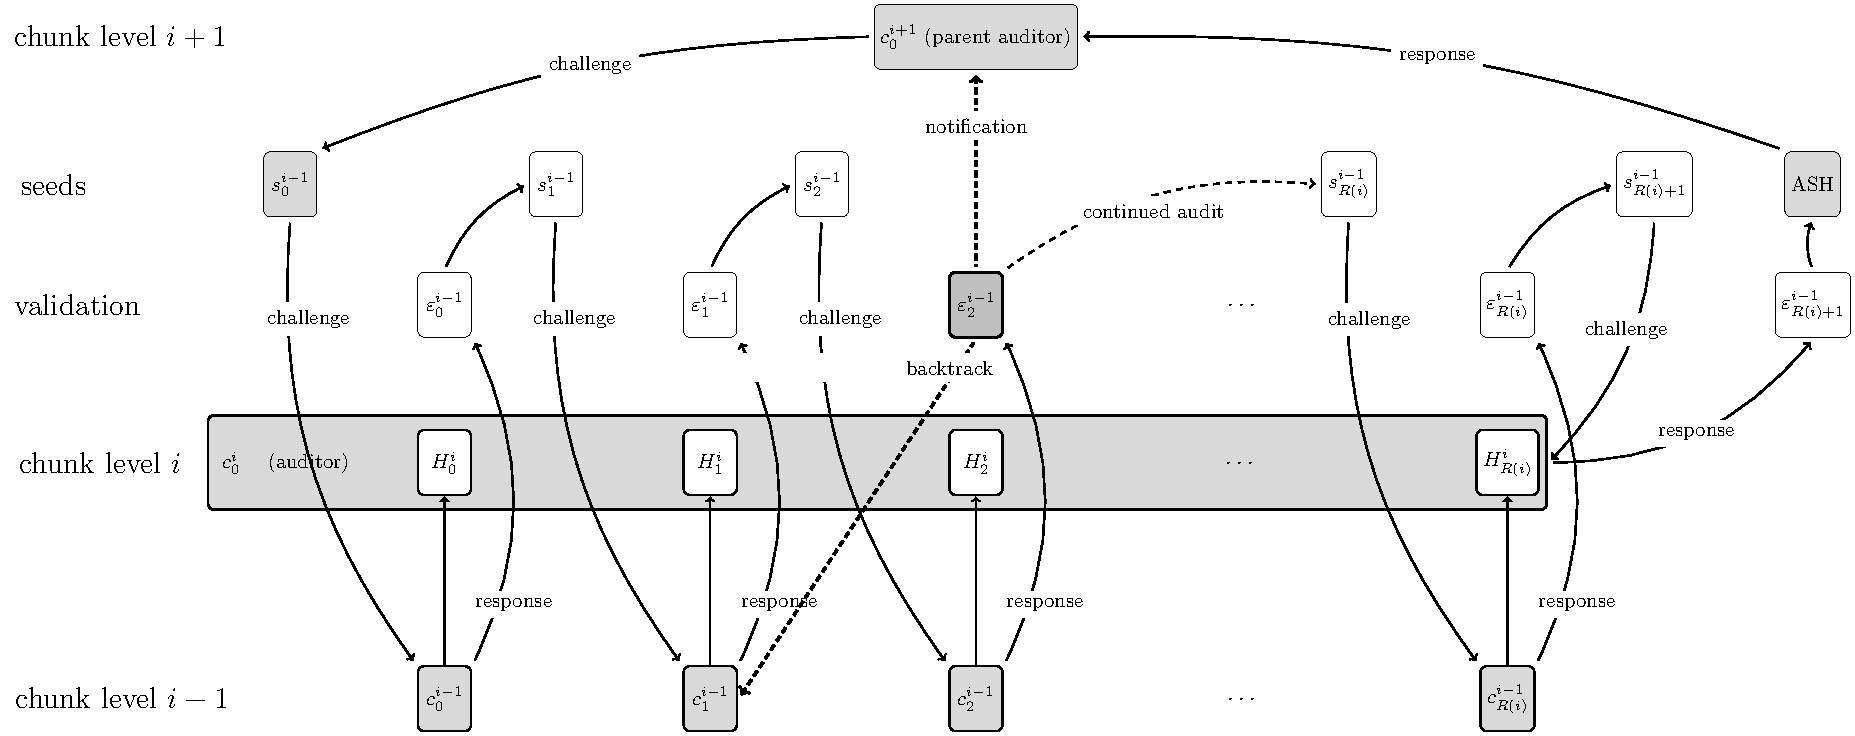
\includegraphics[scale=0.45]{../smash/fig/crash.pdf} % requires the graphicx package
   \caption{This figure zooms in on a chunk in a chunk tree of a document. The chunks represent their custodian nodes that act as auditorqs of the subtree their chunk encodes. The arrows represent the flow of information in the successive steps of calculating CRASH. The custodian of the non-leaf chunk receives a seed and iterates over the hashes of its chunk. It initiates a recursivqe audit challenge on their immediate child nodes. After receiving the response from the chunk's custodian, they perform validation against the error bits and calculate the next seed they then send on to the next child. In case the validation fails, the node backtracks and escalates the audit  to ASH proof challenge    (dashed lines). After piping the seed through the children's audits, it performs a self-challenge as if it was a leaf chunk and sends back the resulting audit secret to their parent auditor.
   }
   \label{fig:crash}
\end{figure}

If the entire audit were to be carried out by just one peer, then chunks for each intermediate node would need to be retrieved in order for the main auditor to initiate all the audit requests for subtrees. Collective auditing has the immediate benefit that no intermediate chunks ever need to be actually retrieved, because the audit of subtrees are carried out by peers that store the chunk. This means a successful audit require only one challenge-response exchange per node involved.
Discounting the one-off task of distributing metadata for the audit which is linear in the size of the collection, the network traffic for each subsequent audit
constitutes a single message roundtrip of a very small constant message.
In the simple context of a trusted system, this can be brought down to hashsize $h$ (32).

Let us assume that given the audit is successful, the probability that the chunk is retrieveably in its full integrity is $p$ and is independent for each chunk.
Calculating the secret itself is on a node is logarithmic in $m$.


Assuming that linear traffic overhead is realistic, the message roundtrip also translates to latency. Since audits are sent to nodes uniformly sampled, the latency is an independent sample. For simplicity we assume that the time used in the recursive network audits simply translates to a constant time factor. If the recursive audit is sequentially organised the time required by audits is linear in the number of nodes which is twice the number of chunks.

Note that partial verification is needed to check non-trusted nodes. In a trusted setup this is not needed and therefore the crash calculation can be massively parallelised on each level. Since the levels are still sequential the time complexity of such a calculation is $log_{b}(n)$.

\section{Integrity audits and erasure coded chunks}

When zooming in on the loss model, we realize that the assumption of a fix probability of a chunk not found is tacitly implying a time interval $d$. Given that the probability of chunks lost we can say the probability that a chunk loss will happen during that period of time. However, if we zoom in to this time period, we realise the individual loss events occur in time. If we somehow detect one and reconstruct it from the rest, it is as if it never happened. This is where we bring in the audits, if audits are carried out multiple times within a time period then it is possible to identify and repair chunks before the damage is too big.
Let us assume that CRASH audits are performed at regular intervals with frequency $f$ during the period $d$ in question. Assuming that the node uses $k$ parity chunks,  a chunk is now irrepairable if and only if all $k$ losses occur during one cycle of audit and repair. Let's derive formally how to set $f$ so that for any file size, the probability that a node is repairable is above a service quality threshold $q$

\begin{align*}
????
\end{align*}

In other words the frequency of audits is set according to the above, then service quality is guaranteed to be at least $q$ irrespective of $s$. The overall resource consumption of the audits are calculated as the following:
It terms of network traffic, it is for the duration of $d$, we send $f\cdot s$ fixed sized roundtrips, which is $O(s^2)$. In terms of time complexity, parallelisation in the trusted case requires it is $O(s\cdot log(s))$ in the trusted scenario and potentially
over the duration of $d$ as $a\cdot f\cdot s$ which is $O(s^2)$.
Of course in order to save the data, we also need to perform repairs on the chunks. Since repair involves fetching the relevant data and recode it,they take way more resources than audits themselves and effectively put a hard limit on the frequency of audits.
As $s$ increases, the speed of repairs won't be able to keep up, i.e., if the time it takes for one chunk to be repairs is longer than $d/f$, we need to resort to increasing $k$ (and $b$) or increasing the chunksize in order to keep the same reliability rate.
Surely this move increases the quadratic component in those cases when the decoding is used, i.e., is every time a retrieval coincides with a repair. Assuming in the worst case that repairs take the full length of the audit, the proportion of nodes needing CRS is the same as the proportion of repairs to audits. This ratio constant. Is it? why?

Note that we reproduced the quadratic complexity, however, we shifted it over to a background process with no real time concern beyond needing to keep up with repairs (on top of computational and network costs) and thereby pushing the range of applicability of erasure codes to include larger files when compared to the original coding used.

\section{Conclusion}

\bibliography{../refs.bib}
\end{document}%% LaTeX - Article customise
